\documentclass[border=10pt]{standalone}

\usepackage{tikz}
\usepackage{tikzsymbols}
\usetikzlibrary{calc,patterns,shapes.geometric}

\def\centerarc[#1](#2)(#3:#4:#5){\draw[#1] ($(#2)+({#5*cos(#3)},{#5*sin(#3)})$) arc (#3:#4:#5);}

\begin{document}
	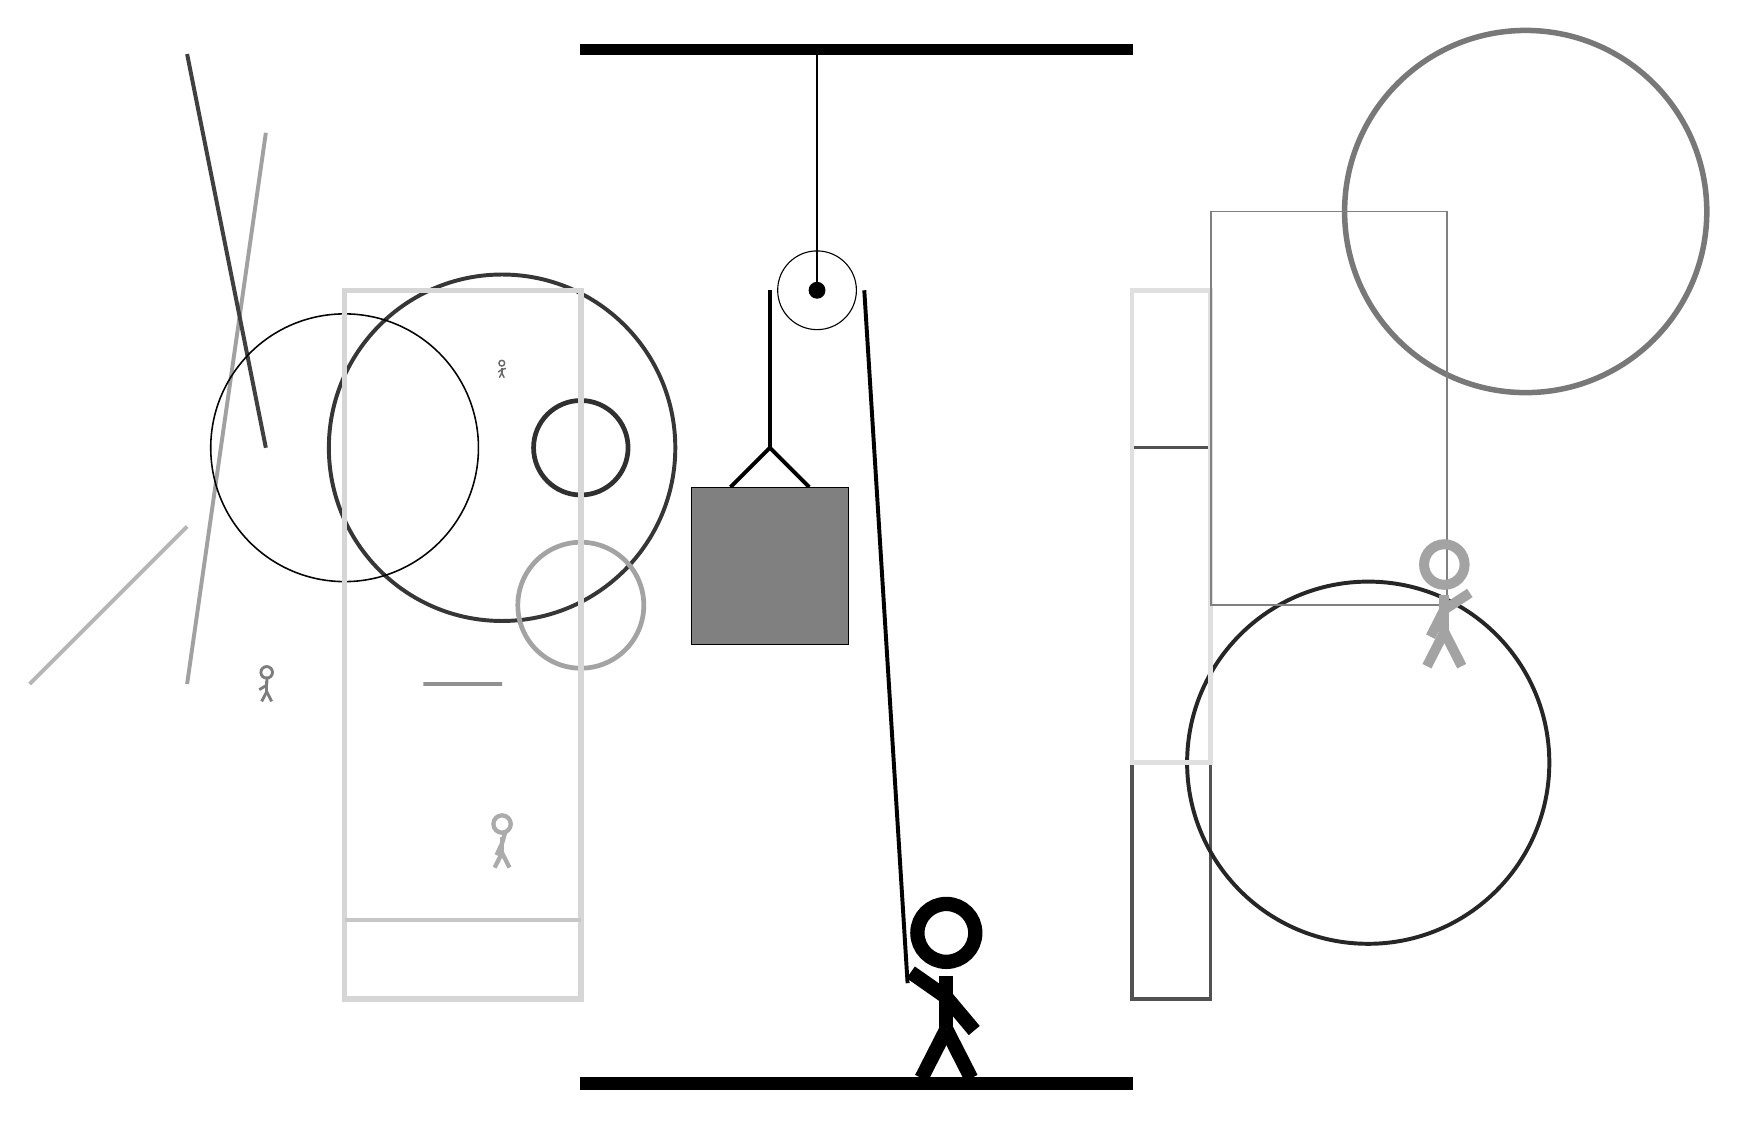
\begin{tikzpicture}
		%%%%% START %%%%%
		
		\draw[fill=black] (-2, 10) rectangle (5, 10.125);
		
		\draw (1, 7) circle (0.5);
		\draw[fill=black] (1, 7) circle (0.1);
		\draw (1, 10) -- (1, 7);
		
		\draw[line width=0.5mm] (-0.1, 4.5) -- (0.4, 5.0) -- (0.9, 4.5);
		\draw[fill=black!50] (-0.6, 4.5) rectangle (1.4, 2.5);
		
		\draw[line width=0.5mm] (0.4, 7) -- (0.4, 5.0);
		\centerarc[line width=0.5mm](1, 7)(0:180:0.6);
		\draw[line width=0.5mm](1.6, 7) -- (2.15, -1.8);
		
		\node at (2.6, -1.9) {\Strichmaxerl[10][-35][-50]};
		
		\draw [line width=0.7mm, color=black!53](10, 8) circle (2.3);
		
		\node[line width=0.2mm, color=black!59] at (-3, 6) {\Strichmaxerl[1][34][17]};
		\draw[line width=0.4mm, color=black!68] (6, 5) rectangle (5, -2);
		\node[line width=0.3mm, color=black!33] at (-3, 0) {\Strichmaxerl[3][65][74]};
		\draw [line width=0.5mm, color=black!85](8, 1) circle (2.3);
		\draw[line width=0.5mm, color=black!37](-6, 9) -- (-7, 2);
		
		\draw [line width=0.6mm, color=black!81](-2, 5) circle (0.6);
		
		\draw[line width=0.5mm, color=black!75](-7, 10) -- (-6, 5);
		\draw[line width=0.5mm, color=black!29](-7, 4) -- (-9, 2);
		\draw [line width=0.5mm, color=black!79](-3, 5) circle (2.2);
		
		\draw[line width=0.6mm, color=black!43] (-3, 2) rectangle (-4, 2);
		\draw[line width=0.6mm, color=black!12] (6, 1) rectangle (5, 7);
		\draw [line width=0.6mm, color=black!36](-2, 3) circle (0.8);
		\draw [line width=0.2mm, color=black!98](-5, 5) circle (1.7);
		\draw[line width=0.2mm, color=black!50] (6, 3) rectangle (9, 8);
		\node[line width=0.4mm, color=black!51] at (-6, 2) {\Strichmaxerl[2][31][87]};
		
		\draw[line width=0.7mm, color=black!16] (-2, 7) rectangle (-5, -2);
		\draw[line width=0.5mm, color=black!22](-5, -1) -- (-2, -1);
		\node[line width=0.4mm, color=black!36] at (9, 3) {\Strichmaxerl[7][63][33]};
		
		\draw[fill=black] (-2, -3) rectangle (5, -3.15);
		
		%%%%% END %%%%%
	\end{tikzpicture}
\end{document}